\documentclass[letterpaper,9pt,twoside,printwatermark=false]{pinp}

%% Some pieces required from the pandoc template
\providecommand{\tightlist}{%
  \setlength{\itemsep}{0pt}\setlength{\parskip}{0pt}}

% Use the lineno option to display guide line numbers if required.
% Note that the use of elements such as single-column equations
% may affect the guide line number alignment.

\usepackage[T1]{fontenc}
\usepackage[utf8]{inputenc}
\usepackage{longtable}

% The geometry package layout settings need to be set here...
\geometry{layoutsize={0.95588\paperwidth,0.98864\paperheight},%
          layouthoffset=0.02206\paperwidth,%
		  layoutvoffset=0.00568\paperheight}

\definecolor{pinpblue}{HTML}{185FAF}  % imagecolorpicker on blue for new R logo
\definecolor{pnasbluetext}{RGB}{101,0,0} %



\title{Assignment 4 - Central Limit Theorem, Confidence Intervals and
Bootstrap. Due October 5, 11:59pm 2018}

\author[a]{EPIB607 - Inferential Statistics}

  \affil[a]{Fall 2018, McGill University}

\setcounter{secnumdepth}{5}

% Please give the surname of the lead author for the running footer
\leadauthor{Bhatnagar and Hanley}

% Keywords are not mandatory, but authors are strongly encouraged to provide them. If provided, please include two to five keywords, separated by the pipe symbol, e.g:
 \keywords{  Sampling distribution |  Standard error |  Normal distribution |  Quantiles |  Percentiles |  Z-scores  }  

\begin{abstract}
In this assignment you will practice calculating confidence intervals.
All graphs and calculations are to be completed in an R Markdown
document using the provided template. You are free to choose any
function from any package to complete the assignment. Concise answers
will be rewarded. Be brief and to the point. Please submit both the
compiled HTML report and the source file (.Rmd) to myCourses by October
5, 2018, 11:59pm. Both HTML and .Rmd files should be saved as
`IDnumber\_LastName\_FirstName\_EPIB607\_A4'.
\end{abstract}

\dates{This version was compiled on \today}
\doi{\url{https://sahirbhatnagar.com/EPIB607/}}

\pinpfootercontents{Assignment 4 due October 5, 2018 by 11:59pm}

\begin{document}

% Optional adjustment to line up main text (after abstract) of first page with line numbers, when using both lineno and twocolumn options.
% You should only change this length when you've finalised the article contents.
\verticaladjustment{-2pt}

\maketitle
\thispagestyle{firststyle}
\ifthenelse{\boolean{shortarticle}}{\ifthenelse{\boolean{singlecolumn}}{\abscontentformatted}{\abscontent}}{}

% If your first paragraph (i.e. with the \dropcap) contains a list environment (quote, quotation, theorem, definition, enumerate, itemize...), the line after the list may have some extra indentation. If this is the case, add \parshape=0 to the end of the list environment.


\section*{Template}\label{template}
\addcontentsline{toc}{section}{Template}

The \texttt{.Rmd} template for Assignment 4 is available
\href{https://github.com/sahirbhatnagar/EPIB607/raw/master/assignments/a4/a4_template.Rmd}{here}

\section{Where do you buy?}\label{where-do-you-buy}

Consumers can purchase nonprescription medications at food stores, mass
merchandise stores such as Kmart and Wal-Mart, or pharmacies. About 45\%
of consumers make such purchases at pharmacies. What accounts for the
popularity of pharmacies, which often charge higher prices?

A study examined consumers' perceptions of overall performance of the
three types of stores, using a long questionnaire that had asked about
such things as ``neat and attractive store'', ``knowledgeable staff'',
and ``assistance in choosing among various types of nonprescription
medication''. A performance score was based on 27 such questions. The
subjects were 201 people chosen at random from the Indianapollis
telephone directory. Here are the means (\(\bar{y}\)) and standard
deviations (\(s\)) of the performances scores for the sample:

\begin{longtable}[]{@{}lll@{}}
\toprule
Store type & \(\bar{y}\) & \(s\)\tabularnewline
\midrule
\endhead
Food stores & 18.67 & 24.95\tabularnewline
Mass merchandisers & 32.38 & 33.37\tabularnewline
Pharmacies & 48.6 & 35.62\tabularnewline
\bottomrule
\end{longtable}

\begin{enumerate}
\def\labelenumi{\alph{enumi}.}
\tightlist
\item
  What population do you think the authors of the study want to draw
  conclusions about?
\item
  What population are you certain they can draw conclusions about?
\item
  Give a 95\% confidence interval for the mean performance for each type
  of store.
\item
  Based on these confidence intervals, are you convinced that consumers
  think that pharmacies offer higher performance than the other types of
  stores?
\end{enumerate}

\section{Deer mice}\label{deer-mice}

Deer mice are small rodents native to North America. Their adult body
lengths (excluding tail) are known to vary approximately Normally, with
mean \(\mu = 86\) millimeters (mm) and standard deviation \(\sigma=8\)
mm. Deer mice are found in diverse habitats and exhibit different
adaptations to their environment. A random sample of 14 deer mice in a
rich forest habitat gives an average body length of \(\bar{y} = 91.1\)
mm. Assume that the standard deviation \(\sigma\) of all deer mice in
this area is also 8 mm.

\begin{enumerate}
\def\labelenumi{\alph{enumi}.}
\tightlist
\item
  What is the standard deviation of the mean length \(\bar{y}\)?
\item
  What critical value do you need to use in order to compute a 95\%
  confidence interval for the mean \(\mu\)
\item
  Give a i) 90\% confidence interval and ii) 95\% confidence interval
  for the mean body length of all deer mice in the forest habitat.
\item
  Why does the 90\% interval have a smaller margin of error?
\end{enumerate}

\section{Does breast-feeding weaken
bones?}\label{does-breast-feeding-weaken-bones}

Breast-feeding mothers secrete calcium into their milk. Some of the
calcium may come from their bones, so mothers may lose bone mineral
content. Researchers compared 47 breast-feeding women with 22 women of
similar age who were neither pregnant nor lactating. They measured the
percent change in the mineral content of the women's spines over three
months. A negative value of \texttt{mineral\_loss} indicates a loss in
mineral content. The data can be read into \texttt{R} and a boxplot
comparing the two groups is shown in the Figure below:

\begin{Shaded}
\begin{Highlighting}[]
\NormalTok{boneloss <-}\StringTok{ }\KeywordTok{read.csv}\NormalTok{(}\StringTok{"https://github.com/sahirbhatnagar/EPIB607/raw/master/data/boneloss.csv"}\NormalTok{)}
\KeywordTok{head}\NormalTok{(boneloss)}
\end{Highlighting}
\end{Shaded}

\begin{ShadedResult}
\begin{verbatim}
#     type mineral_loss
#  1 Other          2.4
#  2 Other          0.0
#  3 Other          0.9
#  4 Other         -0.2
#  5 Other          1.0
#  6 Other          1.7
\end{verbatim}
\end{ShadedResult}

\begin{Shaded}
\begin{Highlighting}[]
\KeywordTok{library}\NormalTok{(mosaic)}
\NormalTok{ggformula}\OperatorTok{::}\KeywordTok{gf_boxplot}\NormalTok{(mineral_loss }\OperatorTok{~}\StringTok{ }\NormalTok{type, }\DataTypeTok{data =}\NormalTok{ boneloss)}
\end{Highlighting}
\end{Shaded}

\begin{center}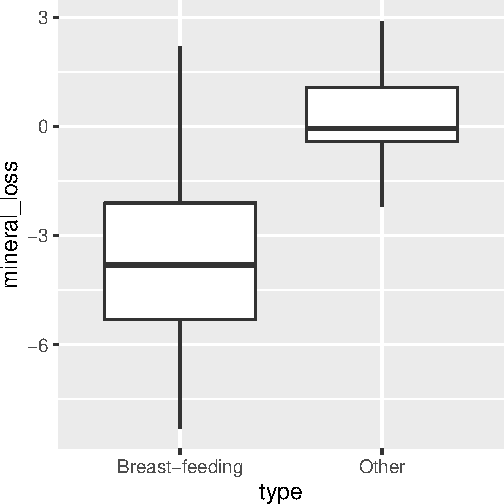
\includegraphics{a4_clt_ci_files/figure-latex/unnamed-chunk-2-1} \end{center}

\begin{enumerate}
\def\labelenumi{\alph{enumi}.}
\tightlist
\item
  Give a 95\% confidence interval for the mean mineral loss for each
  group.
\item
  Based on these confidence intervals, are you convinced that the data
  show distinctly greater bone mineral loss among the breast-feeding
  women?
\item
  (\textbf{BONUS}) Let \(\bar{y}_1\) be the mean mineral loss for
  breast-feeding women and \(\bar{y}_2\) be the mean mineral loss for
  the other group. Construct a 95\% bootstrap confidence interval for
  the difference \(\bar{y}_2 - \bar{y}_1\) based on \(B=10000\)
  bootstrap samples. Interpret this confidence interval and compare it
  to the ones obtained in b. \emph{Hint}: split the data in two
  data.frames by \texttt{type}. For each data.frame, create \(B\)
  resamples and calculate the means for each. Plot the histogram of the
  difference in means, which gives you the bootstrap distribution for
  the difference. From this you can use the \texttt{quantile} function
  to calculate the 95\% CI.
\end{enumerate}

\section{How deep is the ocean?}\label{how-deep-is-the-ocean}

This question is based on the
\href{https://github.com/sahirbhatnagar/EPIB607/blob/master/exercises/water/students/260194225_water_exercise_epib607.pdf}{in-class
Exercise} on sampling distributions. Refer to the
\href{https://github.com/sahirbhatnagar/EPIB607/raw/master/slides/bootstrap/EPIB607_bootstrap.pdf}{slides
on Bootstrap confidence intervals} for \texttt{R} code on how to
calculate bootstrap confidence intervals. For your sample of \(n=20\) of
depths of the ocean, calculate the

\begin{enumerate}
\def\labelenumi{\alph{enumi}.}
\tightlist
\item
  95\% Confidence interval using the \(\pm\) formula
\item
  95\% Confidence interval using the \texttt{qnorm} function
\item
  95\% Confidence interval using \(B=10000\) bootstrap samples
\item
  Plot all three confidence intervals on the same plot and comment on
  the difference/similarities between the 3 intervals. You may use the
  \texttt{compare\_CI} function provided below to produce the plot. This
  takes as input, the sample mean (\texttt{ybar}), and the CIs
  calculated from a,b,c in the form of a numeric vector of length 2 into
  the arguments \texttt{PM}, \texttt{QNORM} and \texttt{BOOT},
  respectively.
\end{enumerate}

\begin{Shaded}
\begin{Highlighting}[]
\NormalTok{compare_CI <-}\StringTok{ }\ControlFlowTok{function}\NormalTok{(ybar, PM, QNORM, BOOT, }
                       \DataTypeTok{col =} \KeywordTok{c}\NormalTok{(}\StringTok{"#E41A1C"}\NormalTok{,}\StringTok{"#377EB8"}\NormalTok{,}\StringTok{"#4DAF4A"}\NormalTok{)) \{}

\NormalTok{  dt <-}\StringTok{ }\KeywordTok{data.frame}\NormalTok{(}\DataTypeTok{type =} \KeywordTok{c}\NormalTok{(}\StringTok{"plus_minus"}\NormalTok{, }\StringTok{"qnorm"}\NormalTok{, }\StringTok{"bootstrap"}\NormalTok{),}
                   \DataTypeTok{ybar =} \KeywordTok{rep}\NormalTok{(ybar, }\DecValTok{3}\NormalTok{),}
                   \DataTypeTok{low =} \KeywordTok{c}\NormalTok{(PM[}\DecValTok{1}\NormalTok{], QNORM[}\DecValTok{1}\NormalTok{], BOOT[}\DecValTok{1}\NormalTok{]),}
                   \DataTypeTok{up =} \KeywordTok{c}\NormalTok{(PM[}\DecValTok{2}\NormalTok{], QNORM[}\DecValTok{2}\NormalTok{], BOOT[}\DecValTok{2}\NormalTok{])}
\NormalTok{  )}
  
  \KeywordTok{plot}\NormalTok{(dt}\OperatorTok{$}\NormalTok{ybar, }\DecValTok{1}\OperatorTok{:}\KeywordTok{nrow}\NormalTok{(dt), }\DataTypeTok{pch =} \DecValTok{20}\NormalTok{, }\DataTypeTok{ylim =} \KeywordTok{c}\NormalTok{(}\DecValTok{0}\NormalTok{, }\DecValTok{5}\NormalTok{), }
       \DataTypeTok{xlim =} \KeywordTok{range}\NormalTok{(}\KeywordTok{pretty}\NormalTok{(}\KeywordTok{c}\NormalTok{(dt}\OperatorTok{$}\NormalTok{low, dt}\OperatorTok{$}\NormalTok{up))),}
       \DataTypeTok{xlab =} \StringTok{'Depth of ocean (m)'}\NormalTok{, }\DataTypeTok{ylab =} \StringTok{'Confidence Interval Type'}\NormalTok{,}
       \DataTypeTok{las =} \DecValTok{1}\NormalTok{, }\DataTypeTok{cex.axis =} \FloatTok{0.8}\NormalTok{, }\DataTypeTok{cex =} \DecValTok{3}\NormalTok{)}
  
  \KeywordTok{abline}\NormalTok{(}\DataTypeTok{v =} \DecValTok{37}\NormalTok{, }\DataTypeTok{lty =} \DecValTok{2}\NormalTok{, }\DataTypeTok{col =} \StringTok{"black"}\NormalTok{, }\DataTypeTok{lwd =} \DecValTok{2}\NormalTok{)}
  \KeywordTok{segments}\NormalTok{(}\DataTypeTok{x0 =}\NormalTok{ dt}\OperatorTok{$}\NormalTok{low, }\DataTypeTok{x1 =}\NormalTok{ dt}\OperatorTok{$}\NormalTok{up,}
           \DataTypeTok{y0 =} \DecValTok{1}\OperatorTok{:}\KeywordTok{nrow}\NormalTok{(dt), }\DataTypeTok{lend =} \DecValTok{1}\NormalTok{,}
           \DataTypeTok{col =}\NormalTok{ col, }\DataTypeTok{lwd =} \DecValTok{4}\NormalTok{)}
  
  \KeywordTok{legend}\NormalTok{(}\StringTok{"topleft"}\NormalTok{,}
         \DataTypeTok{legend =} \KeywordTok{c}\NormalTok{(}\KeywordTok{eval}\NormalTok{(}\KeywordTok{substitute}\NormalTok{( }\KeywordTok{expression}\NormalTok{(}\KeywordTok{paste}\NormalTok{(mu,}\StringTok{" = "}\NormalTok{,}\DecValTok{37}\NormalTok{)))),}
                    \KeywordTok{sprintf}\NormalTok{(}\StringTok{"plus/minus CI: [%.f, %.f]"}\NormalTok{,PM[}\DecValTok{1}\NormalTok{], PM[}\DecValTok{2}\NormalTok{]),}
                    \KeywordTok{sprintf}\NormalTok{(}\StringTok{"qnorm CI: [%.f, %.f]"}\NormalTok{,QNORM[}\DecValTok{1}\NormalTok{], QNORM[}\DecValTok{2}\NormalTok{]),}
                    \KeywordTok{sprintf}\NormalTok{(}\StringTok{"bootstrap CI: [%.f, %.f]"}\NormalTok{,BOOT[}\DecValTok{1}\NormalTok{], BOOT[}\DecValTok{2}\NormalTok{])),}
         \DataTypeTok{lty =} \KeywordTok{c}\NormalTok{(}\DecValTok{1}\NormalTok{, }\DecValTok{1}\NormalTok{,}\DecValTok{1}\NormalTok{,}\DecValTok{1}\NormalTok{),}
         \DataTypeTok{col =} \KeywordTok{c}\NormalTok{(}\StringTok{"black"}\NormalTok{,col), }\DataTypeTok{lwd =} \DecValTok{4}\NormalTok{)}
\NormalTok{\}}

\CommentTok{# example of how to use the function:}
\KeywordTok{compare_CI}\NormalTok{(}\DataTypeTok{ybar =} \DecValTok{36}\NormalTok{, }\DataTypeTok{PM =} \KeywordTok{c}\NormalTok{(}\DecValTok{28}\NormalTok{, }\DecValTok{40}\NormalTok{), }\DataTypeTok{QNORM =} \KeywordTok{c}\NormalTok{(}\DecValTok{25}\NormalTok{,}\DecValTok{40}\NormalTok{), }\DataTypeTok{BOOT =} \KeywordTok{c}\NormalTok{(}\DecValTok{31}\NormalTok{, }\DecValTok{38}\NormalTok{))}
\end{Highlighting}
\end{Shaded}

%\showmatmethods


\bibliography{pinp}
\bibliographystyle{jss}



\end{document}

